\chapter{Survey}
\label{chap:2} 

\section{All methods}
In this chapter there will be a brief description of some papers that treated \textit{brain classification}. We can divide the methods in the several techniques that the papers use to build the brain classification: Deep Learning, Statistical Fingerprints and Machine Learning. Also, to compare them, and find a possible good way to make brain classification, some have been tested. The results are in chapter \ref{chap:3}.

\subsection{Deep Learning}
\paragraph{GroupINN: Grouping-based Interpretable Neural Network for Classification of Limited, Noisy Brain Data}\
\\

This paper of Yan Y. et al \cite{groupinn} proposes a grouping-based interpretable neural network model, GroupINN, that classifies cognitive performance with 85\% fewer parameters than baseline deep models, while also identifying the most predictive brain subnetworks within several task-specific contexts. In the design of the neural network is included the idea of node grouping. In this way the model learns the node grouping and extracts the graph features jointly.
\\

The problem statement of this paper is: given a set of subjects, each with corresponding fMRI data and a label associated with a certain phenotype, we seek to devise an efficient, interpretable, and parsimonious neural network model that can predict each phenotype with high accuracy.
\\

To reduce the number of parameters used in the model, they adopted the idea of multi-graph clustering (where the goal is to find a common clustering across multiple graphs) to summarize the original graph into a supergraph with each cluster as a supernode. 
\\

The neural network is formed by three different types of layers: node grouping layer, graph convolutional layer and fully connected layer. The node grouping layer is designed to “hide” the non-indicative (‘noisy’) edges by grouping them into a cluster, thus highlighting the indicative edges: two nodes are assigned to different groups if their connection is identified as important.
Graph convolutional layers are used to capture the structure of the supergraph.
\\

The neural network is also divided in two branches, one processes the positive graphs and one the negative ones. 
All in all, the architecture consists of three kinds of layers and two branches. 
The input graph is the correlation matrix $W$. The first layer is a dimensionality reduction layer and the output is a matrix $W^{s}$ representing the supergraph. Following the dimensionality reduction layer, three graph convolutional layers are used. At last, the positive and negative outputs of the previous layer are concatenated, flattened and sent to the fully connected layer (with softmax activation).
\begin{figure}[htbp]
	\centering
	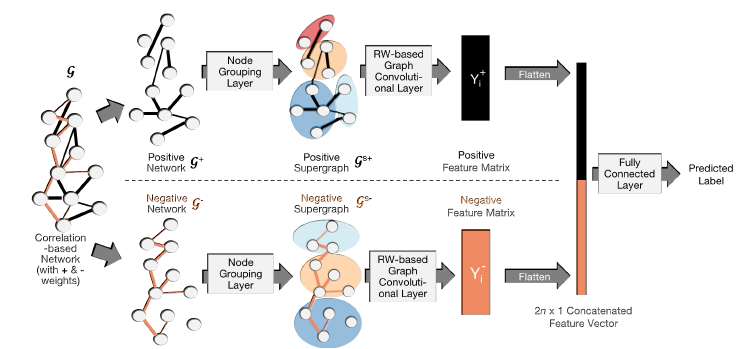
\includegraphics[scale=0.8]{Immagini/Groupinn1.PNG}
	\caption{\label{fig:diagram5}}
\end{figure}
\\

Regarding the experimentation part, they used a dataset taken from Human Connectome Project 1200 (HCPt) \cite{hcp}. 
This dataset consists of 966 subjects to which has been measured brain activity, through fMRI, while they were performing specific tasks. The four task-based datasets used in this experiment are: \textit{Emotion, Gambling, Social} and \textit{Working Memory}. It is divided in 90\% train/validation set and 10\% testing set. For the evaluation they take in consideration \textit{accuracy} and the \textit{runtime}. Comparing their method, they found out that it is faster and with less parameters than other works, so it is more interpretable, as well as having good accuracy.
\\

\paragraph{Deep Learning-based Pipeline to Recognize Alzheimer’s Disease using fMRI Data}
\paragraph{Functional Brain Network Classification for Alzheimer’s Disease Detection with Deep Features and Extreme Learning Machine}

\subsection{Statistical Fingerprints}
\paragraph{Explainable Classification of Brain Networks via Contrast Subgraphs}\
\\

In this paper they introduce an approach for classifying brain networks based on extracting contrast subgraphs, i.e., a set of vertices whose induced subgraphs are dense in one class of graphs and sparse in the other. The model is extremely simple, with just one parameter, excellent interpretability and good classification accuracy. 
\\
They exploited contrast subgraph TD-ASD (the subgraph that maximizes the difference between the number of edges in the class TD, typically developed brains, with respect to the same measure for class ASD, people with autism spectrum deseas). Vertex size represents the importance of the vertex in discriminating the two classes. In fact they ended up with some important rules:
1. If an individual exhibits more than 62 edges among the 15 vertices of the contrast subgraph ASD-TD, then there are high chances that the individual is affected by ASD; 2. If the number of edges induced by the contrast subgraph ASD-TD is smaller than half of the number of edges induced by the contrast subgraph TD-ASD, then there are high chances that the individual is not affected by ASD. 3. If the number of edges induced by the contrast subgraph ASD-TD is smaller than the number of edges induced by the contrast subgraph TD-ASD, then there are high chances that the individual is affected by ASD.
\\
Each individual is represented by an undirected unweighted graph with $|V|$ = 116 vertices.
\paragraph{Unsupervised Network Embedding for Graph Visualization, Clustering and Classification}
\paragraph{Supervised classification of structural brain networks reveals gender differences}
\paragraph{Sub-network Kernels for Measuring Similarity of Brain Connectivity Networks in Disease Diagnosis}
\paragraph{Integration Of Network Topological Features And Graph Fourier Transform For Fmri Data Analysis}

\subsection{Machine Learning}
\paragraph{Network Classification With Applications To Brain Connectomics}
\paragraph{Stable Biomarker Identification For Predicting Schizophrenia in the Human Connectome}

\paragraph{Multi-modality disease modelling via collective deep matrix factorization}